%%%%%%%%%%%%%%%%%%%%%%%%%%%%%%%%%%%%%%%%%%%%%%%%%%%%%%%%%%%%%%%%%%%%%%
% How to use writeLaTeX: 
%
% You edit the source code here on the left, and the preview on the
% right shows you the result within a few seconds.
%
% Bookmark this page and share the URL with your co-authors. They can
% edit at the same time!
%
% You can upload figures, bibliographies, custom classes and
% styles using the files menu.
%
%%%%%%%%%%%%%%%%%%%%%%%%%%%%%%%%%%%%%%%%%%%%%%%%%%%%%%%%%%%%%%%%%%%%%%

\documentclass[12pt]{article}

\usepackage{sbc-template}

\usepackage{graphicx,url}

\usepackage[brazil]{babel}   
\usepackage[utf8]{inputenc}  

     
\sloppy

\title{Instructions for Authors of SBC Conferences\\ Papers and Abstracts}

\author{Luciana P. Nedel\inst{1}, Rafael H. Bordini\inst{2}, Flávio Rech
  Wagner\inst{1}, Jomi F. Hübner\inst{3} }


\address{Instituto de Informática -- Universidade Federal do Rio Grande do Sul
  (UFRGS)\\
  Caixa Postal 15.064 -- 91.501-970 -- Porto Alegre -- RS -- Brazil
\nextinstitute
  Department of Computer Science -- University of Durham\\
  Durham, U.K.
\nextinstitute
  Departamento de Sistemas e Computação\\
  Universidade Regional de Blumenal (FURB) -- Blumenau, SC -- Brazil
  \email{\{nedel,flavio\}@inf.ufrgs.br, R.Bordini@durham.ac.uk,
  jomi@inf.furb.br}
}

\begin{document} 

\maketitle
     
\begin{resumo} 
  Este meta-artigo descreve o estilo a ser usado na confecção de artigos e
  resumos de artigos para publicação nos anais das conferências organizadas
  pela SBC. É solicitada a escrita de resumo e abstract apenas para os artigos
  escritos em português. Artigos em inglês deverão apresentar apenas abstract.
  Nos dois casos, o autor deve tomar cuidado para que o resumo (e o abstract)
  não ultrapassem 10 linhas cada, sendo que ambos devem estar na primeira
  página do artigo.
\end{resumo}

\section{Introdução}

\section{Desenvolvimento}

\section{Resultados}

Nesta seção, apresentamos os resultados obtidos de nossa implementação. Inicialmente, analisamos a equivalência lógica entre os códigos sequencial e paralelo, considerando possíveis erros que podem surgir na paralelização, como condições de corrida ou inconsistências de sincronização. Em seguida, ilustramos, por meio de mapas de calor, a atualização dos valores da matriz ao longo do tempo. Por fim, realizamos uma análise comparativa dos tempos médios de execução, \textit{speedup} e eficiência entre as duas versões.

\subsection{Validação da Implementação}

Para assegurar a correção das duas implementações, verificamos em cada iteração se os valores presentes em cada célula da matriz são idênticos. Dessa forma, o resultado final na última iteração deve ser o mesmo em ambas as versões.

Por meio desse procedimento, utilizando a interface Python em conjunto com um Jupyter Notebook, comprovamos que as duas soluções produzem resultados idênticos. Isso era esperado, pois no código paralelo não ocorrem condições de corrida, uma vez que a escrita não é realizada na mesma região de memória das leituras, tornando o processamento de cada célula pelas \textit{threads} independente.

\subsection{Validação da Implementação}

Para ilustrar o funcionamento da implementação, foram gerados mapas de calor, representado pela Figura \ref{fig:heatmap}, nos quais cada ponto de uma matriz 50x50 é representado por uma cor distinta. Cores escuras correspondem a valores próximos de um, indicando alta concentração do contaminante, enquanto cores claras representam valores próximos de zero, indicando baixa presença de contaminação.

\begin{figure}[ht]
\centering
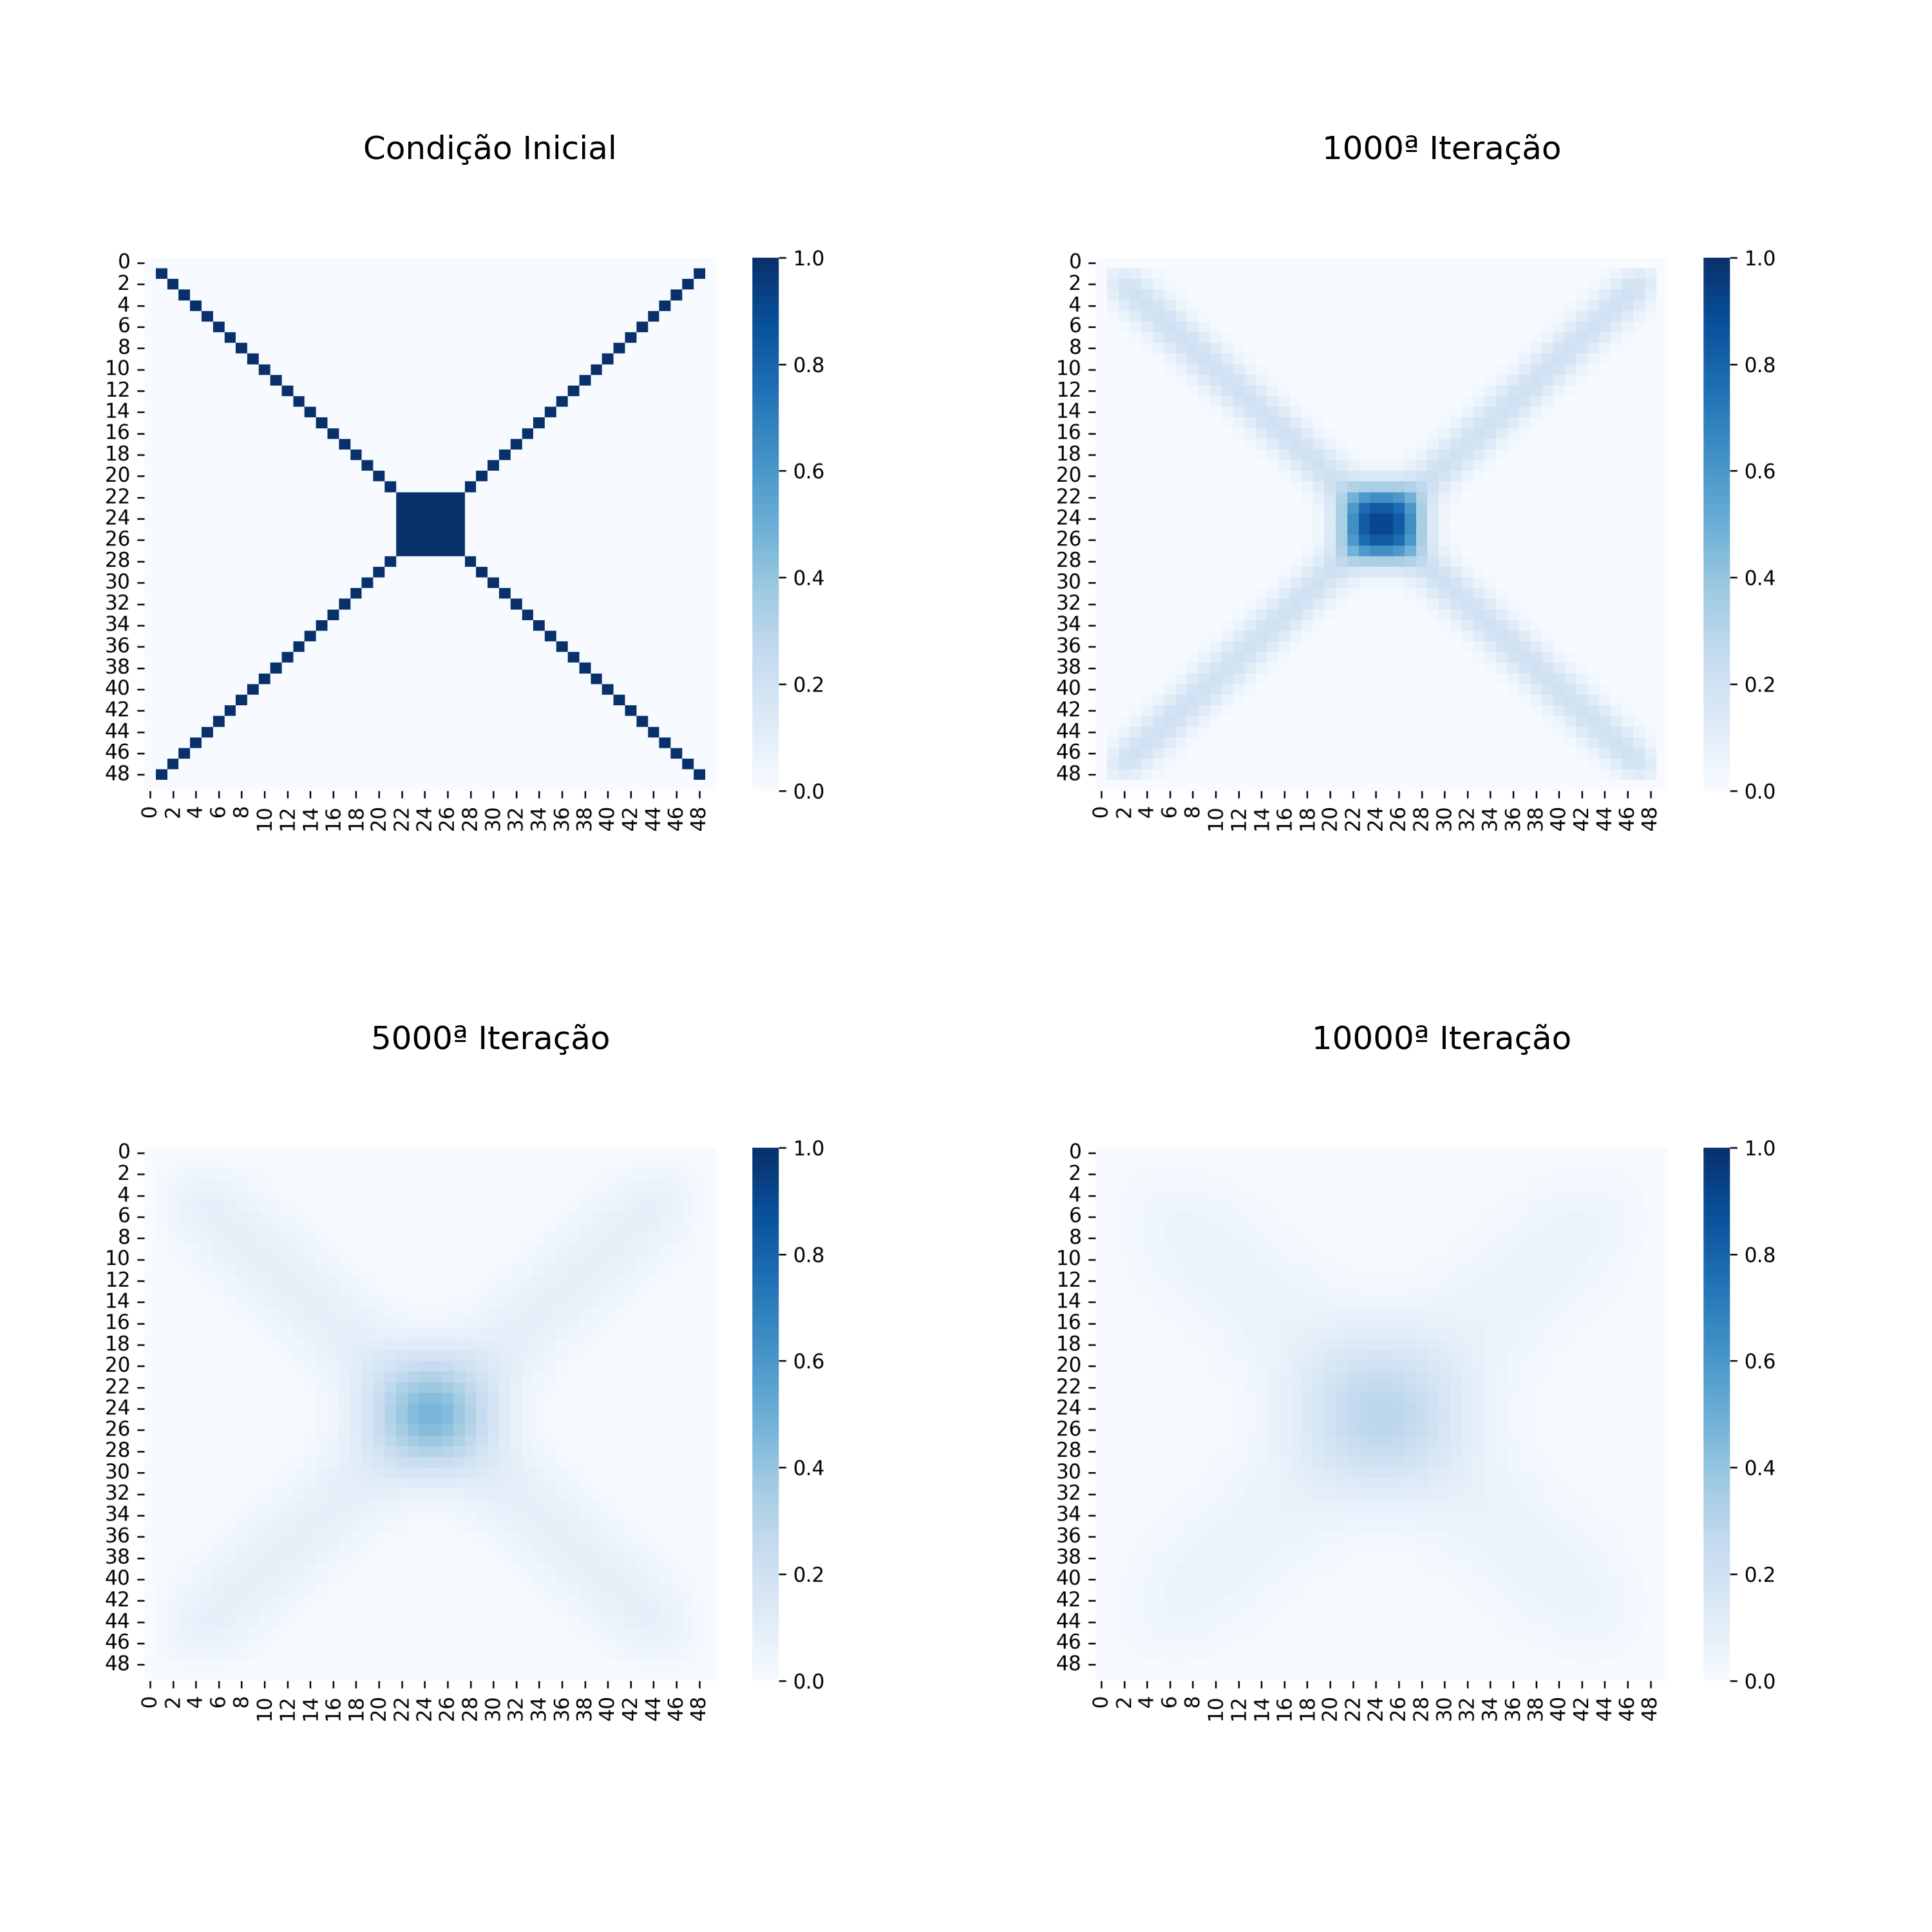
\includegraphics[width=.7\textwidth]{figs/heatmap.png}
\caption{Mapa de calor em quatro instantes distintos da simulação.}
\label{fig:heatmap}
\end{figure}

Analisando a progressão dos mapas de calor, observamos que o comportamento faz sentido no contexto da solução proposta. Inicialmente, o contaminante é adicionado com alta concentração nas diagonais e no centro da matriz, evidenciado pelas regiões azuis escuras. Com o avanço das iterações, o contaminante começa a se difundir para as regiões adjacentes, aumentando gradativamente a luminosidade nessas áreas e diminuindo nos pontos de concentração inicial. Na última iteração, a concentração se distribui uniformemente pela matriz, com valores próximos entre si.

\subsection{Análise de Desempenho}

A análise de desempenho foi realizada em um computador \textit{desktop} com as seguintes especificações. Além disso, as especificações dos parâmetros do problema foram incluídas na tabela correspondente.

\begin{table}[ht]
\centering
\caption{Tabela de especificação de Hardware}
\vspace{0.3cm}
\begin{tabular}{||c c||} 
 \hline
Especificações & Detalhes \\ [0.5ex] 
 \hline\hline
 Processador & Intel i7-4790 @ 3.60GHz \\ 
 \hline
 Núcleos / Lógicos & 4 / 8  \\
 \hline
 Memória RAM & 8 GB  \\
 \hline
 Sistema Operacional & Ubuntu 22.04.05 (via WSL)   \\ 
 \hline
\end{tabular}
\end{table}

\begin{table}[ht]
\centering
\caption{Tabela de especificação da Simulação}
\vspace{0.3cm}
\begin{tabular}{||c c||} 
 \hline
Especificações & Detalhes \\ [0.5ex] 
 \hline\hline
 Dimensão da Matriz (N x N) & 2000 x 2000 \\ 
 \hline
 Número de Iterações & 500  \\
 \hline
 Distribuição Inicial & Alta concentração no centro  \\
 \hline
 Coeficiente de Difusão & 0.1   \\ 
 \hline
 dt & 0.01   \\ 
 \hline
 dx & 1.0   \\ 
 \hline
\end{tabular}
\end{table}

Para obter valores mais consistentes e minimizar influências externas, como outros programas em execução, cada teste foi executado quinze vezes e, assim, calculamos o tempo médio gasto e seu desvio padrão. O \textit{speedup} é calculado dividindo-se o tempo de execução sequencial pelo tempo de execução paralelo correspondente, enquanto a eficiência é determinada ao dividir o \textit{speedup} pelo número de \textit{threads} utilizados.

\begin{table}[ht]
\centering
\caption{Tabela de comparação de desempenho entre o código sequencial e o paralelo utilizando OpenMP.}
\vspace{0.3cm}
\begin{tabular}{||c c c c||} 
 \hline
 Nº Threads & Tempo & Speedup & Eficiência \\ [0.5ex] 
 \hline\hline
 1 & 26.22 $\pm$ 2.09 & 1.0 & 100\% \\ 
 \hline
 2 & 14.59 $\pm$ 1.49 & 1.80 & 89,88\% \\
 \hline
 4 & 10.60 $\pm$ 1.43 & 2.47 & 61.82\% \\
 \hline
 8 & 8.52 $\pm$ 1.32 & 3.08 & 38.48\% \\
 \hline
 16 & 8.29 $\pm$ 1.29 & 3.16 & 19.77\% \\
 \hline
 32 & 8.67 $\pm$ 1.43 & 3.03 & 9.45\% \\ 
 \hline
\end{tabular}
\end{table}

\begin{figure}[ht]
\centering
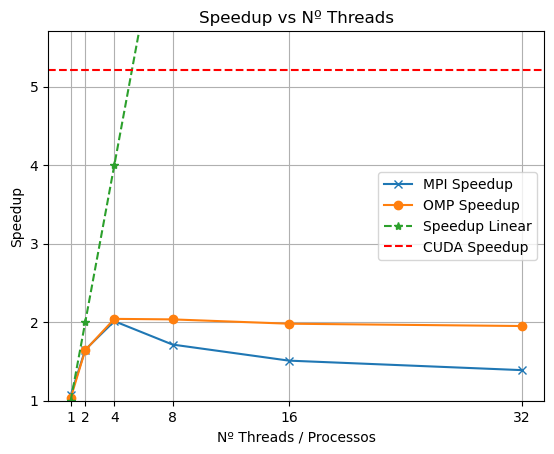
\includegraphics[width=.5\textwidth]{figs/speedupxthreads.png}
\caption{Gráfico do \textit{speedup} por número de \textit{threads}}
\label{fig:speedupOMP}
\end{figure}

\begin{figure}[ht]
\centering
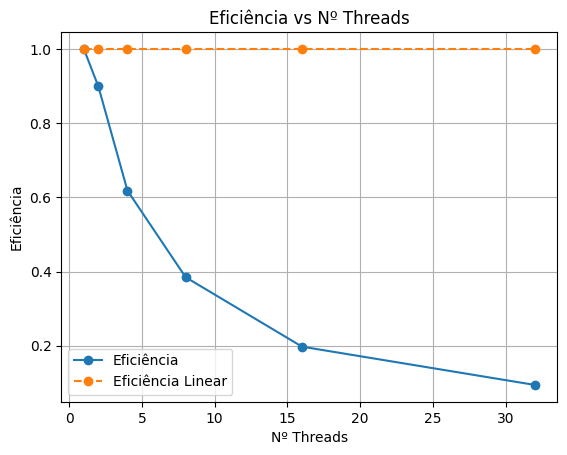
\includegraphics[width=.5\textwidth]{figs/eficienciaxthreads.png}
\caption{Gráfico da eficiência por número de \textit{threads}}
\label{fig:eficienciaOMP}
\end{figure}


O gráfico de \textit{speedup} (Figura \ref{fig:speedupOMP}) mostra uma tendência de estabilização em torno do valor três, enquanto o \textit{speedup} linear ideal apresenta valores significativamente maiores, o que pode sugerir que a escalabilidade da aplicação é limitada, possivelmente devido a \textit{overheads} de sincronização ou ao fato de que o problema não é suficientemente grande para aproveitar eficientemente um número maior de \textit{threads}. Além disso, o desempenho pode estar sendo afetado pela latência de memória ou pela arquitetura do processador utilizado e, consequentemente, não há grandes vantagens em utilizar um número elevado de \textit{threads} para resolver este problema específico, já que aumentaria excessivamente o consumo de energia pela máquina, que pode ser observado pela grande queda no gráfico de eficiência da Figura \ref{fig:eficienciaOMP}.

\section{Conclusão}

\section{General Information}

All full papers and posters (short papers) submitted to some SBC conference,
including any supporting documents, should be written in English or in
Portuguese. The format paper should be A4 with single column, 3.5 cm for upper
margin, 2.5 cm for bottom margin and 3.0 cm for lateral margins, without
headers or footers. The main font must be Times, 12 point nominal size, with 6
points of space before each paragraph. Page numbers must be suppressed.

Full papers must respect the page limits defined by the conference.
Conferences that publish just abstracts ask for \textbf{one}-page texts.

\section{First Page} \label{sec:firstpage}

The first page must display the paper title, the name and address of the
authors, the abstract in English and ``resumo'' in Portuguese (``resumos'' are
required only for papers written in Portuguese). The title must be centered
over the whole page, in 16 point boldface font and with 12 points of space
before itself. Author names must be centered in 12 point font, bold, all of
them disposed in the same line, separated by commas and with 12 points of
space after the title. Addresses must be centered in 12 point font, also with
12 points of space after the authors' names. E-mail addresses should be
written using font Courier New, 10 point nominal size, with 6 points of space
before and 6 points of space after.

The abstract and ``resumo'' (if is the case) must be in 12 point Times font,
indented 0.8cm on both sides. The word \textbf{Abstract} and \textbf{Resumo},
should be written in boldface and must precede the text.

\section{CD-ROMs and Printed Proceedings}

In some conferences, the papers are published on CD-ROM while only the
abstract is published in the printed Proceedings. In this case, authors are
invited to prepare two final versions of the paper. One, complete, to be
published on the CD and the other, containing only the first page, with
abstract and ``resumo'' (for papers in Portuguese).

\section{Sections and Paragraphs}

Section titles must be in boldface, 13pt, flush left. There should be an extra
12 pt of space before each title. Section numbering is optional. The first
paragraph of each section should not be indented, while the first lines of
subsequent paragraphs should be indented by 1.27 cm.

\subsection{Subsections}

The subsection titles must be in boldface, 12pt, flush left.

\section{Figures and Captions}\label{sec:figs}


Figure and table captions should be centered if less than one line
(Figure~\ref{fig:exampleFig1}), otherwise justified and indented by 0.8cm on
both margins, as shown in Figure~\ref{fig:exampleFig2}. The caption font must
be Helvetica, 10 point, boldface, with 6 points of space before and after each
caption.

\begin{figure}[ht]
\centering
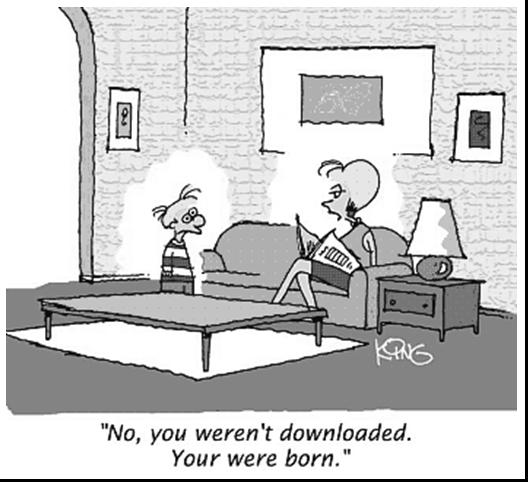
\includegraphics[width=.5\textwidth]{fig1.jpg}
\caption{A typical figure}
\label{fig:exampleFig1}
\end{figure}

\begin{figure}[ht]
\centering
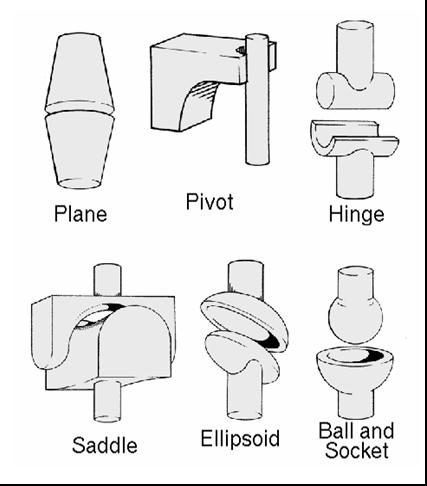
\includegraphics[width=.3\textwidth]{fig2.jpg}
\caption{This figure is an example of a figure caption taking more than one
  line and justified considering margins mentioned in Section~\ref{sec:figs}.}
\label{fig:exampleFig2}
\end{figure}

In tables, try to avoid the use of colored or shaded backgrounds, and avoid
thick, doubled, or unnecessary framing lines. When reporting empirical data,
do not use more decimal digits than warranted by their precision and
reproducibility. Table caption must be placed before the table (see Table 1)
and the font used must also be Helvetica, 10 point, boldface, with 6 points of
space before and after each caption.

\begin{table}[ht]
\centering
\caption{Variables to be considered on the evaluation of interaction
  techniques}
\label{tab:exTable1}
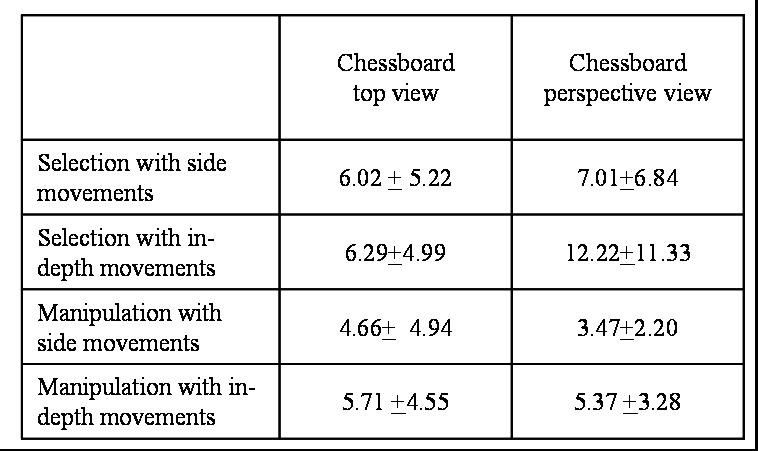
\includegraphics[width=.7\textwidth]{table.jpg}
\end{table}


\section{Images}

All images and illustrations should be in black-and-white, or gray tones,
excepting for the papers that will be electronically available (on CD-ROMs,
internet, etc.). The image resolution on paper should be about 600 dpi for
black-and-white images, and 150-300 dpi for grayscale images.  Do not include
images with excessive resolution, as they may take hours to print, without any
visible difference in the result. 

\section{References}

Bibliographic references must be unambiguous and uniform.  We recommend giving
the author names references in brackets, e.g. \cite{knuth:84},
\cite{boulic:91}, and \cite{smith:99}.

The references must be listed using 12 point font size, with 6 points of space
before each reference. The first line of each reference should not be
indented, while the subsequent should be indented by 0.5 cm.

\bibliographystyle{sbc}
\bibliography{sbc-template}

\end{document}
